\section{矩阵的基本运算}

\subsection{矩阵的概念}

\begin{definition}[矩阵]
    由 $m\times n$ 个数 $a_{ij}~ (i=1,2,\cdots,m;j=1,2,\cdots,n)$ 按一定次序排成的 $m$
    行 $ n $ 列的矩形数表
    $$\begin{pNiceArray}{cccc}
            a_{11}  & a_{12}  & \cdots & a_{1 n} \\
            a_{21}  & a_{22}  & \cdots & a_{2 n} \\
            \vdots  & \vdots  &        & \vdots  \\
            a_{m 1} & a_{m 2} & \cdots & a_{m n}
        \end{pNiceArray}$$
    称为 $ m \times n $ 矩阵 ($m $ 行 $ n $ 列矩阵), $a_{i j} $ 叫做矩阵的元素, 矩阵可简记为
    $$\vb*{A}=\left(a_{i j}\right)_{m \times n} \text { 或 } \vb*{A}=\left(a_{i j}\right) \text {. }$$
    当 $ m=n $ 时, 即矩阵的行数与列数相同时, 称 $ \vb*{A} $ 为 $ n $ 阶方阵;
    当 $ m=1 $ 时, 矩阵只有一行, 称为行矩阵, 记为
    $$\vb*{A}=\left(a_{11}, a_{12}, \cdots, a_{1 n}\right)$$
    这样的行矩阵也称为 $ n $ 维行向量;
    当 $ n=1 $ 时, 矩阵只有一列, 称为列矩阵, 记为
    $$\vb*{A}=\begin{pNiceArray}{c}
            a_{11} \\
            a_{21} \\
            \vdots \\
            a_{m 1}
        \end{pNiceArray}$$
    这样的列矩阵也称为 $ m $ 维列向量.
\end{definition}

\begin{definition}[矩阵的负]
    矩阵 $ \vb*{A} $ 中各元素变号得到的矩阵叫做 $ \vb*{A} $ 的负矩阵, 
    记作 $ -\vb*{A} $, 即
    $$-\vb*{A}=\left(-a_{i j}\right)_{m \times n} \text {. }$$
\end{definition}

\begin{definition}[零矩阵]
    如果矩阵 $\vb*{A}$ 的所有元素都是 $0$, 即
    $$\vb*{A}=\begin{pNiceArray}{cccc}
            0      & 0      & \cdots & 0      \\
            0      & 0      & \cdots & 0      \\
            \vdots & \vdots &        & \vdots \\
            0      & 0      & \cdots & 0
        \end{pNiceArray},$$
    则 $\vb*{A}$ 称为零矩阵, 记为 $\vb*{O}$.
\end{definition}

\begin{definition}[单位矩阵]
    主对角线上元素都是 1, 其余元素均为零的方阵称为单位矩阵, 记为 $ \vb*{E}$ (或 $ \vb*{I} $), 即
    $$\vb*{E}=\begin{pNiceArray}{cccc}
            1      & 0      & \cdots & 0      \\
            0      & 1      & \cdots & 0      \\
            \vdots & \vdots & \ddots & \vdots \\
            0      & 0      & \cdots & 1
        \end{pNiceArray} .$$
\end{definition}

\begin{definition}[数量矩阵]
    主对角线上元素为任意常数, 而主对角线外的元素均为零的矩阵. 若对角矩阵的主对角线上的元素相等, 则称为数量矩阵.
\end{definition}

\begin{definition}[三角形矩阵]
    主对角线下方元素全为零的方阵称为上三角形矩阵; 主对角线上方元素全为零的方阵称为下三角形矩阵; 上、下三角形矩阵统称为三角形矩阵.
\end{definition}

\begin{definition}[矩阵的转置]
    把矩阵 $ \vb*{A}=\left(a_{i j}\right)_{m \times n} $ 的行列互换而得到的矩阵 $ \left(a_{j i}\right)_{n \times m} $ 称为 $ \vb*{A} $ 的转置矩阵, 
    记为 $ \vb*{A}^{\top} $ (或 $ \vb*{A}^{\prime} $).
\end{definition}

\begin{definition}[对称矩阵]
    如果 $ n $ 阶方阵 $ \vb*{A}=\left(a_{i j}\right) $ 满足 $ a_{i j}=a_{j i}~ (i, j=1,2, \cdots, n) $, 即 $ \vb*{A}^{\top}=\vb*{A} $, 则称 $ \vb*{A} $ 为对称矩阵.
\end{definition}
\begin{definition}[反对称矩阵]
    如果 $ n $ 阶方阵 $ \vb*{A}=\left(a_{i j}\right) $ 满足 $ a_{i j}=-a_{j i}~ (i \neq j),~a_{i i}=0~ (i, j=1,2, \cdots ,  n) $, 
    即 $ \vb*{A}^{\top}=-\vb*{A} $, 则称 $ \vb*{A} $ 为反对称矩阵.
\end{definition}
\begin{theorem}[方阵的对称表达]
    任意 $n$ 阶方阵都可以表示成一个对称方阵与一个反对称方阵的和.
\end{theorem}
\begin{proof}[{\songti \textbf{证}}]
    设 $\vb*{A}$ 为任意 $n$ 阶方阵, 令 $\vb*{B}=\dfrac{1}{2}\qty(\vb*{A}+\vb*{A}^{\top}),~\vb*{C}=\dfrac{1}{2}\qty(\vb*{A}-\vb*{A}^{\top})$, 则 
    $$\vb*{B}^\top=\dfrac{1}{2}\qty(\vb*{A}+\vb*{A}^{\top})^\top=\dfrac{1}{2}\qty(\vb*{A}+\vb*{A}^{\top})=B,~
    \vb*{C}^\top=\dfrac{1}{2}\qty(\vb*{A}-\vb*{A}^{\top})^\top=\dfrac{1}{2}\qty(\vb*{A}^\top-\vb*{A})=-\vb*{C}$$
    即 $\vb*{B}$ 为对称矩阵, $\vb*{C}$ 为反对称矩阵, 显然 $\vb*{A}=\vb*{B}+\vb*{C}$.
\end{proof}

\begin{definition}[正交矩阵]
    对方阵 $ \vb*{A} $, 如果有 $ \vb*{A}^{\top} \vb*{A}=\vb*{A} \vb*{A}^{\top}=\vb*{E} $, 则称 $ \vb*{A} $ 为正交矩阵.
\end{definition}
\begin{theorem}[正交矩阵的行列式]
    若方阵 $ \vb*{A} $ 为正交矩阵, 那么 $|\vb*{A}|=\pm 1.$
\end{theorem}
\begin{proof}[{\songti \textbf{证}}]
    $1=\det\vb*{E}=\det\qty(\vb*{A}^\top\vb*{A})=\det\qty(\vb*{A}^\top)\det\vb*{A}=\det^2\vb*{A}\Rightarrow \det\vb*{A}=\pm 1.$
\end{proof}

\begin{example}
    已知 $\vb*{A}$ 是 4 阶正交矩阵且 $|\vb*{A}|<0$, $\vb*{B}$ 是 4 阶矩阵, 若 $|\vb*{B}-\vb*{A}|=5$, 求 $\qty|\vb*{E}-\vb*{AB}^\top|.$
\end{example}
\begin{solution}
    因为 $\vb*{AA}^\top=\vb*{A}^\top\vb*{A}=\vb*{E}$, 所以 $|\vb*{A}|=\pm 1$, 又 $|\vb*{A}|<0$, 即 $|\vb*{A}|=-1$, 
    \begin{flalign*}
        \qty|\vb*{E}-\vb*{AB}^\top|=\qty|\vb*{AA}^\top-\vb*{AB}^\top|=|\vb*{A}|\qty|(\vb*{A}-\vb*{B})^\top|=-|\vb*{A}-\vb*{B}|=-|-(\vb*{B}-\vb*{A})|=-(-1)^4|\vb*{B}-\vb*{A}|=-5.
    \end{flalign*}
\end{solution}

\begin{definition}[幂零矩阵]
    对方阵 $ \vb*{A} $, 如果存在正整数 $ m $, 使 $ \vb*{A}^{m}=\mathbf{0} $, 则称 $ \vb*{A} $ 为幂零矩阵.
\end{definition}

\begin{definition}[幂等矩阵]
    满足 $ \vb*{A}^{2}=\vb*{A} $ 的方阵 $ \vb*{A} $ 称为幂等矩阵.
\end{definition}

\begin{definition}[对合矩阵]
    满足 $ \vb*{A}^{2}=\vb*{E} $ 的方阵 $ \vb*{A} $ 称为对合矩阵.
\end{definition}

\begin{definition}[方阵的行列式]
    方阵 $ \vb*{A} $ 的元素按原来的位置构成的行列式, 称为方阵 $ \vb*{A} $ 的行列式, 记为 $ |\vb*{A}| $.
\end{definition}

\begin{example}
    设矩阵 $\vb*{A}$ 是 3 阶方阵, 且 $$|\vb*{A}-2\vb*{E}|=|\vb*{A}-3\vb*{E}|=|\vb*{A}-4\vb*{E}|=3$$
    求 $|\vb*{A}-\vb*{E}|.$
\end{example}
\begin{solution}
    设 $f(x)=|\vb*{A}-x\vb*{E}|=\mqty|a_{11}-x&a_{12}&a_{13}\\a_{21}&a_{22}-x&a_{23}\\a_{31}&a_{32}&a_{33}-x|$, 那么 $f(x)$ 一定是以 $x$ 为变量的首项系数为 $-1$ 的三次多项式, 又
    $$|\vb*{A}-2\vb*{E}|=|\vb*{A}-3\vb*{E}|=|\vb*{A}-4\vb*{E}|=3$$
    所以 $f(x)=-(x-2)(x-3)(x-4)+3$, 那么 $|\vb*{A}-\vb*{E}|=f(1)=9.$
\end{solution}

\begin{definition}[奇异矩阵与非奇异矩阵]
    若 $ |\vb*{A}|=0 $, 称 $ \vb*{A} $ 为奇异矩阵, 否则称为非奇异矩阵.
\end{definition}

\begin{definition}[矩阵的迹]
    设有 $n$ 阶方阵 $\vb*{A}$, 那么 $\vb*{A}$ 的迹定义为 $\displaystyle\mathrm{tr}\vb*{A}=\sum_{k=1}^{n}a_{kk}$.
\end{definition}
\begin{theorem}[迹的相关性质]
    又设 $\vb*{B}\in M_n(K),~\lambda\in K$, 则
    \setcounter{magicrownumbers}{0}
    \begin{table}[H]
        \centering
        \begin{tabular}{l l}
            (\rownumber)$\tr(\vb*{A}+\vb*{B})=\tr (\vb*{A})+\tr(\vb*{B})$ & (\rownumber)$\tr\qty(\vb*{A}^{\top})=\tr (\vb*{A})$   \\
            \midrule
            (\rownumber)$\tr(\vb*{AB})=\tr(\vb*{BA})$                     & (\rownumber)$\tr(\lambda\vb*{A})=\lambda\tr(\vb*{A})$
        \end{tabular}
    \end{table}
\end{theorem}

\subsection{矩阵的运算}

\textbf{矩阵的运算公式}
\setcounter{magicrownumbers}{0}
\begin{table}[H]
    \centering
    \begin{tabular}{l l}
        关于矩阵的加法运算公式                                                                                                                         \\
        (\rownumber) $\vb*{A}+\vb*{B}=\vb*{B}+\vb*{A}$             & (\rownumber) $(\vb*{A}+\vb*{B})+\vb*{C}=\vb*{A}+(\vb*{B}+\vb*{C})$                \\
        (\rownumber) $\vb*{A}+(-\vb*{A})=\mathbf{0}$               & (\rownumber) $(\vb*{A}-\vb*{B})=\vb*{A}+(-\vb*{B})$                               \\
        \midrule
        关于数乘运算的公式                                                                                                                             \\
        (\rownumber) $(k l) \vb*{A}=k(l \vb*{A})$                  & (\rownumber) $(k+l) \vb*{A}=k \vb*{A}+l \vb*{A} $                                 \\
        (\rownumber) $k(\vb*{A}+\vb*{B})=k \vb*{A}+k \vb*{B}$                                                                                          \\
        \midrule
        关于矩阵乘法运算的公式                                                                                                                         \\
        (\rownumber) $(\vb*{A B}) \vb*{C}=\vb*{A}(\vb*{B C})$      & (\rownumber) $k(\vb*{A} \vb*{B})=(k \vb*{A}) \vb*{B}=\vb*{A}(k \vb*{B})$          \\
        (\rownumber) $\vb*{A}(\vb*{B}+\vb*{C})=\vb*{AB}+\vb*{AC}$  & (\rownumber) $(\vb*{B}+\vb*{C})\vb*{A}=\vb*{BA}+\vb*{CA}$                         \\
        (\rownumber) $\vb*{E A}=\vb*{A} \vb*{E}=\vb*{A}$           & (\rownumber) $(\lambda \vb*{E}) \vb*{A}=\lambda \vb*{A}=\vb*{A}(\lambda \vb*{E})$ \\
        (\rownumber) $\vb*{A}^{k} \vb*{A}^{l}=\vb*{A}^{k+l}$       & (\rownumber) $\left(\vb*{A}^{k}\right)^{l}=\vb*{A}^{k l}$                         \\
        \midrule
        关于矩阵转置运算的公式                                                                                                                         \\
        (\rownumber) $\left(\vb*{A}^{\top}\right)^{\top}=\vb*{A} $ & (\rownumber) $(\vb*{A}+\vb*{B})^{\top}=\vb*{A}^{\top}+\vb*{B}^{\top} $            \\
        (\rownumber) $(k \vb*{A})^{\top}=k \vb*{A}^{\top}$         & (\rownumber) $(\vb*{A B})^{\top}=\vb*{B}^{\top} \vb*{A}^{\top}$                   \\
        \midrule
        \multicolumn{2}{l}{关于方阵的行列式的公式, 若 $ \vb*{A}, \vb*{B} $ 是 $ n $ 阶方阵, 则}                                                        \\
        (\rownumber) $\left|\vb*{A}^{\top}\right|=|\vb*{A}|$       & (\rownumber) $|\lambda \vb*{A}|=\lambda^{n}|\vb*{A}|$                             \\
        (\rownumber) $|\vb*{A B}|=|\vb*{A}||\vb*{B}|$              & (\rownumber) $|\vb*{A B}|=|\vb*{B A}| $
    \end{tabular}
\end{table}
需要注意的事项:
\begin{enumerate}[label=(\arabic{*})]
    \item 矩阵的乘法一般不满足交换律, 即 $ \vb*{A B} $ 有意义, 但 $ \vb*{B A} $ 不一定有意义; 即使 $ \vb*{A B} $ 和 $ \vb*{B A} $ 都有意义, 两者也不一定相等.
    \item 两个非零矩阵相乘, 可能是零矩阵, 从而不能从 $ \vb*{A B}=\mathbf{0} $ 推出 $ \vb*{A}=\mathbf{0} $ 或 $ \vb*{B}=\mathbf{0} $.
    \item 矩阵的乘法一般不满足消去律, 即不能从 $ \vb*{A C}=\vb*{B} \vb*{C} $ 推出 $ \vb*{A}=\vb*{B} .$
\end{enumerate}

\begin{definition}[矩阵相等]
    设 $$\vb*{A}=\left(a_{i j}\right)_{m \times n}, \vb*{B}=\left(b_{i j}\right)_{m \times n}$$
    如果 $ a_{i j}=b_{i j}~ (i=1,2, \cdots, m ; j=1,2, \cdots, n) $, 则称矩阵 $ \vb*{A} $ 与 $ \vb*{B} $ 相等, 记作 $ \vb*{A}=\vb*{B}.$
\end{definition}

\begin{definition}[矩阵加减]
    设 $$\vb*{A}=\left(a_{i j}\right)_{m \times n}, \vb*{B}=\left(b_{i j}\right)_{m \times n}, \vb*{C}=\left(c_{i j}\right)_{m \times n}$$
    其中 $ c_{i j}=a_{i j} \pm b_{i j}~ (i=1,2, \cdots, m ; j=1,2, \cdots, n) $, 则称 $ \vb*{C} $ 为矩阵 $ \vb*{A} $ 与 $ \vb*{B} $ 的和 (或差), 
    记为 $ \vb*{C}=\vb*{A} \pm \vb*{B}. $
\end{definition}

\begin{definition}[矩阵数乘]
    设 $ k $ 为一个常数, $$\vb*{A}=\left(a_{i j}\right)_{m \times n}, ~  \vb*{C}=\left(c_{i j}\right)_{m \times n}$$
    其中 $ c_{i j}=k a_{i j}~ (i=1,2, \cdots, m ; j=1,2, \cdots, n) $, 则称矩阵 $ \vb*{C} $ 为数 $ k $ 与矩阵 $ \vb*{A} $ 的数量乘积, 
    简称数乘, 记为 $ k \vb*{A} .$
\end{definition}

\begin{definition}[矩阵乘法]
    设 $ \vb*{A}=\left(a_{i j}\right)_{m \times s}, \vb*{B}=\left(b_{i j}\right)_{s \times n}, \vb*{C}=\left(c_{i j}\right)_{m \times n} $, 
    其中 $$c_{i j}=\sum_{l=1}^{s} a_{i l} b_{l j}~ (i=1,2, \cdots, m ; j=1,2, \cdots, n)$$
    则称矩阵 $ \vb*{C} $ 为矩阵 $ \vb*{A} $ 与 $ \vb*{B} $ 的乘积, 
    记为 $ \vb*{AB} $, 即 $ \vb*{C}=\vb*{AB} .$
\end{definition}

\begin{figure}[H]
    \centering
    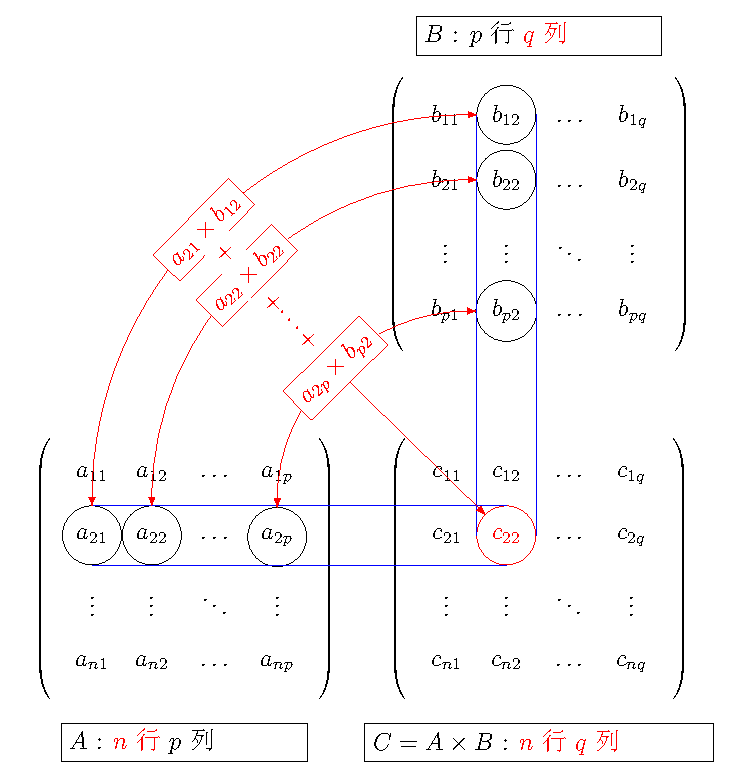
\includegraphics[scale=0.75]{figures/matrix-multiplication.pdf}
    \caption{}
\end{figure}

\begin{example}
    设 $\vb*{A}=\begin{pmatrix}
            a_{11} & a_{12} \\
            a_{21} & a_{22} \\
            a_{31} & a_{32} \\
        \end{pmatrix}$, 
    $\vb*{B}=\begin{pmatrix}
            b_1 & 0   \\
            0   & b_2
        \end{pmatrix}$, 
    $\vb*{C}=\begin{pmatrix}
            c_1 & 0   & 0   \\
            0   & c_2 & 0   \\
            0   & 0   & c_3
        \end{pmatrix}$, 求 $\vb*{AB}$ 和 $\vb*{CA}$.
\end{example}
\begin{solution}
    $\vb*{AB}=\begin{pmatrix}
            a_{11} & a_{12} \\
            a_{21} & a_{22} \\
            a_{31} & a_{32} \\
        \end{pmatrix}\begin{pmatrix}
            b_1 & 0   \\
            0   & b_2
        \end{pmatrix}=\begin{pmatrix}
            a_{11}b_1 & a_{12}b_2 \\
            a_{21}b_1 & a_{22}b_2 \\
            a_{31}b_1 & a_{32}b_2
        \end{pmatrix}$; 同理
    $\vb*{CA}=\begin{pmatrix}
            c_1a_{11} & c_1a_{12} \\
            c_2a_{21} & c_2a_{22} \\
            c_3a_{31} & c_3a_{32}
        \end{pmatrix}$
\end{solution}

\begin{example}
    设 $\vb*{A}$ 是 4 阶方阵, $\vb*{B}$ 是 5 阶方阵, 且 $|\vb*{A}|=2,|\vb*{B}|=-2$, 求 $|-|\vb*{A}|\vb*{B}|$ 与 $|-|\vb*{B}|\vb*{A}|$.
\end{example}
\begin{solution}
    $|-|\vb*{A}|\vb*{B}|=|-2\vb*{B}|=(-2)^{5}|\vb*{B}|=64$, $|-|\vb*{B}|\vb*{A}|=|2\vb*{A}|=2^4|\vb*{A}|=32.$
\end{solution}

\begin{example}
    设 $\vb*{A},~\vb*{B}$ 均为 3 阶矩阵, 满足 $\vb*{AB}+2\vb*{A}+\vb*{B}+\vb*{E}=\vb*{O}$, 
    若 $|\vb*{B}|=\mqty|1&2&0\\1&2&0\\1&2&1|$, 求 $|\vb*{A}+\vb*{E}|.$
\end{example}
\begin{solution}
    对 $\vb*{AB}+2\vb*{A}+\vb*{B}+2\vb*{E}$ 使用多项式除法, 得 $$\vb*{AB}+2\vb*{A}+\vb*{B}+2\vb*{E}=(\vb*{A}+\vb*{E})(\vb*{B}+2\vb*{E})=\vb*{E}\Rightarrow|\vb*{A}+\vb*{E}|=\dfrac{1}{|\vb*{B}+2\vb*{E}|}=\dfrac{1}{30}.$$
\end{solution}

\begin{example}
    (2021 数二) 已知矩阵 $\vb*{A}=\begin{pmatrix}
            1  & 0  & -1 \\
            2  & -1 & 1  \\
            -1 & 2  & -5
        \end{pmatrix}$, 若存在下三角可逆矩阵 $\vb*{P}$ 和上三角可逆矩阵 $\vb*{Q}$, 
    使 $\vb*{PAQ}$ 为对角矩阵, 求 $\vb*{P}$ 和 $\vb*{Q}$.
\end{example}
\begin{solution}
    对 $\vb*{A}$ 做初等行变换, 化为上三角矩阵 $\vb*{B}$, 
    \begin{flalign*}
        \begin{pNiceArray}{c:c}
            \vb*{A} & \vb*{E}
        \end{pNiceArray} & =\begin{pNiceArray}{ccc:ccc}
                                1  & 0  & -1 & 1 & 0 & 0 \\
                                2  & -1 & 1  & 0 & 1 & 0 \\
                                -1 & 2  & -5 & 0 & 0 & 1 \\
                            \end{pNiceArray}\xrightarrow[r_3+r_1]{r_2-2r_1}
        \begin{pNiceArray}{ccc:ccc}
            1 & 0  & -1 & 1  & 0 & 0 \\
            0 & -1 & 3  & -2 & 1 & 0 \\
            0 & 2  & -6 & 1  & 0 & 1 \\
        \end{pNiceArray}                                                   \\
                                & \xrightarrow[]{r_3+2r_2}\begin{pNiceArray}{ccc:ccc}
                                                              1 & 0  & -1 & 1  & 0 & 0 \\
                                                              0 & -1 & 3  & -2 & 1 & 0 \\
                                                              0 & 0  & 0  & -3 & 2 & 1 \\
                                                          \end{pNiceArray}
        \xrightarrow[]{}\begin{pNiceArray}{ccc:ccc}
                            1 & 0 & -1 & 1  & 0  & 0 \\
                            0 & 1 & -3 & 2  & -1 & 0 \\
                            0 & 0 & 0  & -3 & 2  & 1 \\
                        \end{pNiceArray}=\begin{pNiceArray}{c:c}
                                             \vb*{B} & \vb*{P}
                                         \end{pNiceArray}
    \end{flalign*}
    所以 $\vb*{P}=\begin{pmatrix}
            1  & 0  & 0 \\
            2  & -1 & 0 \\
            -3 & 2  & 1
        \end{pmatrix}$, 再对 $\vb*{B}$ 作列变换 (或 $\vb*{B}^{\top}$ 作行变换) 化为对角矩阵, 可求得 $\vb*{Q}$ (或 $\vb*{Q}^{\top}$)
    $$\begin{pNiceArray}{c}
            \vb*{B} \\
            \hdottedline
            \vb*{E}
        \end{pNiceArray}=\begin{pNiceArray}{ccc}
            1 & 0 & -1 \\
            0 & 1 & -3 \\
            0 & 0 & 0  \\
            \hdottedline
            1 & 0 & 0  \\
            0 & 1 & 0  \\
            0 & 0 & 1
        \end{pNiceArray}\xrightarrow[c_3+3c_1]{c_3+c_1}\begin{pNiceArray}{ccc}
            1 & 0 & 0 \\
            0 & 1 & 0 \\
            0 & 0 & 0 \\
            \hdottedline
            1 & 0 & 1 \\
            0 & 1 & 3 \\
            0 & 0 & 1
        \end{pNiceArray}$$
    可得 $\vb*{Q}=\begin{pmatrix}
            1 & 0 & 1 \\
            0 & 1 & 3 \\
            0 & 0 & 1
        \end{pmatrix}.$
    或 $$\begin{pNiceArray}{c:c}
            \vb*{B}^{\top} & \vb*{E}
        \end{pNiceArray}=\begin{pNiceArray}{ccc:ccc}
            1  & 0  & 0 & 1 & 0 & 0 \\
            0  & 1  & 0 & 0 & 1 & 0 \\
            -1 & -3 & 0 & 0 & 0 & 1 \\
        \end{pNiceArray}\xrightarrow[r_3+r_1]{r_3+3r_2}
        \begin{pNiceArray}{ccc:ccc}
            1 & 0 & 0 & 1 & 0 & 0 \\
            0 & 1 & 0 & 0 & 1 & 0 \\
            0 & 0 & 0 & 1 & 3 & 1 \\
        \end{pNiceArray}$$
    得 $\vb*{Q}^{\top}=\begin{pmatrix}
            1 & 0 & 0 \\
            0 & 1 & 0 \\
            1 & 3 & 1
        \end{pmatrix}.$
\end{solution}

\subsection{Carlson 不等式及其应用}

\begin{theorem}[Carlson 不等式]
    对于 $n\times m$ 矩阵
    $$\begin{pmatrix}
            a_{11} & a_{12} & \dots  & a_{1m} \\
            a_{21} & a_{22} & \dots  & a_{2m} \\
            \vdots & \vdots & \ddots & \vdots \\
            a_{n1} & a_{n2} & \dots  & a_{nm} \\
        \end{pmatrix}$$
    其中 $a_{ij}\geqslant0~ (i=1,2,\cdots,n,j=1,2,\cdots,m)$, 则
    $$\qty[\prod_{j=1}^{m}\qty(\sum_{i=1}^{n}a_{ij})]^{\frac{1}{m}}\geqslant \sum_{i=1}^{n}\qty(\prod_{j=1}^{m}a_{ij})^{\frac{1}{m}}$$
    其中, 等号成立的充要条件是至少有一列数都是 0 或所有行中的数对应成比例.
\end{theorem}
\begin{proof}[{\songti \textbf{证}}]
    记 $\displaystyle A_j = \sum_{i=1}^{n}a_{ij}~ (j=1,2,\cdots,m),~G_j=\prod_{j=1}^{m}a_{ij}~ (i=1,2,\cdots,n)$, 
    若某个 $A_j=0$, 则由 $a_{ij}\geqslant 0~ (i=1,2,\cdots,n)$, 得 $$a_{1j}=a_{2j}=\cdots=a_{nj}=0$$
    此时, $G_1=G_2=\cdots=G_n=0$, 从而 $$\qty[\prod_{j=1}^{m}\qty(\sum_{i=1}^{n}a_{ij})]^{\frac{1}{m}}=\sum_{i=1}^{n}\qty(\prod_{j=1}^{m}a_{ij})^{\frac{1}{m}}$$
    若所有 $A_j>0$, 由均值不等式得 $$\dfrac{a_{i1}}{A_1}+\dfrac{a_{i2}}{A_2}+\cdots+\dfrac{a_{im}}{A_m}\geqslant m\qty(\dfrac{\displaystyle\prod_{j=1}^{m}a_{ij}}{\displaystyle\prod_{j=1}^{m}A_j})^{\frac{1}{m}}~ (i=1,2,\cdots,n)$$
    将以上 $n$ 个不等式相加得
    $$m\geqslant m\sum_{i=1}^{n}\qty(\dfrac{\displaystyle\prod_{j=1}^{m}a_{ij}}{\displaystyle\prod_{j=1}^{m}A_j})^{\frac{1}{m}}=m\dfrac{\displaystyle\sum_{i=1}^{n}G_i^{\frac{1}{m}}}{\qty(\displaystyle\prod_{j=1}^{m}A_j)^{\frac{1}{m}}}$$
    等号成立的充要条件是至少有一列数都是 0 或 $\dfrac{a_{i1}}{A_1}=\dfrac{a_{i2}}{A_2}=\cdots=\dfrac{a_{im}}{A_m}$.
\end{proof}

\begin{example}
    已知 $a,b,c>0$, 证明: $$\qty(a^2+ab+b^2)\qty(b^2+bc+c^2)\qty(c^2+ca+a^2)\geqslant (ab+bc+ca)^3.$$
\end{example}
\begin{proof}[{\songti \textbf{证}}]
    构造 $3\times 3$ 矩阵
    $$\begin{pmatrix}
            a^2 & c^2 & ca  \\
            ab  & b^2 & a^2 \\
            b^2 & bc  & c^2
        \end{pmatrix}$$
    由 Carlson 不等式得证.
\end{proof}

\begin{example}
    已知 $a,b,c>0$, $a^2+b^2+c^2=14$, 求证: $a^5+\dfrac{b^5}{8}+\dfrac{c^5}{27}\geqslant 14.$
\end{example}
\begin{proof}[{\songti \textbf{证}}]
    构造 $3\times 5$ 矩阵
    $$\begin{pmatrix}
            a^5             & a^5             & 1 & 1 & 1 \\[6pt]
            \dfrac{b^5}{8}  & \dfrac{b^5}{8}  & 4 & 4 & 4 \\[6pt]
            \dfrac{c^5}{27} & \dfrac{c^5}{27} & 9 & 9 & 9
        \end{pmatrix}$$
    由 Carlson 不等式得, 
    \begin{flalign*}
        \qty[\qty(a^5+\dfrac{b^5}{8}+\dfrac{c^5}{27})^2(1+4+9)^3]^{\frac{1}{5}} & \geqslant \qty(a^5\cdot a^5\cdot 1^3)^{\frac{1}{5}}+\qty(\dfrac{b^5}{8}\cdot \dfrac{b^5}{8}\cdot 4^3)^{\frac{1}{5}}+\qty(\dfrac{c^5}{27}\cdot\dfrac{c^5}{27}\cdot 9^3)^{\frac{1}{5}} \\
        \qty[\qty(a^5+\dfrac{b^5}{8}+\dfrac{c^5}{27})^214^3]^{\frac{1}{5}}      & \geqslant a^2+b^2+c^2=14
    \end{flalign*}
    整理得证 $a^5+\dfrac{b^5}{8}+\dfrac{c^5}{27}\geqslant 14.$
\end{proof}

\begin{example}
    已知 $a_i>0~ (i=1,2,\cdots,n),~n\geqslant 2$, 且 $\displaystyle\sum_{i=1}^{n}a_i=1$, 
    证明: $\displaystyle\sum_{i=1}^{n}\dfrac{a_i}{2-a_i}\geqslant \dfrac{n}{2n-1}.$
\end{example}
\begin{proof}[{\songti \textbf{证}}]
    原不等式等价为 $$\sum_{i=1}^{n}\dfrac{2}{2-a_i}\geqslant \dfrac{2n^2}{2n-1}$$
    为此, 构造 $n\times 2$ 矩阵
    $$\begin{pmatrix}
            \dfrac{2}{2-a_1} & 2-a_1  \\[6pt]
            \dfrac{2}{2-a_2} & 2-a_2  \\[6pt]
            \vdots           & \vdots \\[6pt]
            \dfrac{2}{2-a_n} & 2-a_n
        \end{pmatrix}$$
    由 Carlson 不等式得, 
    \begin{flalign*}
        \qty[\qty(\sum_{i=1}^{n}\dfrac{2}{2-a_i})\sum_{i=1}^{n}(2-a_i)]^{\frac{1}{2}}\geqslant \sqrt{2}n\Rightarrow\qty(\sum_{i=1}^{n}\dfrac{2}{2-a_i})(2n-1)\geqslant 2n^2
    \end{flalign*}
    整理得证 $\displaystyle\sum_{i=1}^{n}\dfrac{a_i}{2-a_i}\geqslant \dfrac{n}{2n-1}.$
\end{proof}

\begin{example}
    (第 36 届 IMO) 设 $a,b,c>0$, 且 $abc=1$, 证明: $\dfrac{1}{a^3(b+c)}+\dfrac{1}{b^3(c+a)}+\dfrac{1}{c^3(a+b)}\geqslant\dfrac{3}{2}.$
\end{example}
\begin{proof}[{\songti \textbf{证}}]
    原不等式等价为 $$\dfrac{b^2c^2}{a(b+c)}+\dfrac{a^2c^2}{b(c+a)}+\dfrac{a^2b^2}{c(a+b)}$$
    构造 $3\times 2$ 矩阵
    $$\begin{pmatrix}
            \dfrac{b^2c^2}{a(b+c)} & a(b+c) \\[6pt]
            \dfrac{a^2c^2}{b(a+c)} & b(a+c) \\[6pt]
            \dfrac{a^2b^2}{c(a+b)} & c(a+b)
        \end{pmatrix}$$
    由 Carlson 不等式得, 
    \begin{flalign*}
        \qty{\qty[\dfrac{b^2c^2}{a(b+c)}+\dfrac{a^2c^2}{b(c+a)}+\dfrac{a^2b^2}{c(a+b)}]\cdot2(ab+bc+ca)}^{\frac{1}{2}} & \geqslant ab+bc+ca                                                                      \\
        \dfrac{b^2c^2}{a(b+c)}+\dfrac{a^2c^2}{b(c+a)}+\dfrac{a^2b^2}{c(a+b)}                                           & \geqslant \dfrac{1}{2}(ab+bc+ca)\geqslant \dfrac{3}{2}\sqrt[3]{a^2b^2c^2}=\dfrac{3}{2}.
    \end{flalign*}
\end{proof}